La parte cruciale del progetto \emph{PathS} si basa sulla gestione delle informazioni aggiuntive relative ai percorsi pedonali e la possibilità di sfruttarle per fornire un servizio alternativo agli utenti finali. La persistenza, la gestione e l'elaborazione di questi dati avviene nella componente \emph{server}. 
In questo capitolo saranno presentati i requisiti individuati per assolvere allo scopo del progetto e il modo in cui questi requisiti hanno guidato la definizione dell'architettura del software da sviluppare.

\section{Requisiti}
Come per l'altra componente, anche nel caso del server si è preso spunto dalla precedente versione del progetto (\emph{Path2.0}) e si è cercato di identificarne i limiti per poter essere adattato al nuovo contesto e agli scopi più ampi che sono stati definiti. Le situazioni e le interrogazioni a cui si intende applicare il progetto sono del tipo:
\begin{itemize}
\item qual è il percorso meno rumoroso in quest’ora del giorno?
\item che percorso devo seguire per ottenere il maggior numero di tratti all’ombra?
\item quali sono i percorsi preferiti dagli utenti che hanno visitato questa zona?
\end{itemize}
Le risposte fornite dovranno sempre tenere conto della soddisfabilità della domanda (quindi fornire sempre un percorso valido) ma valutare anche le preferenze espresse dall’utente.

Dal punto di vista tecnologico la soluzione precedente è stata valutata non idonea coma base di partenza, in particolare presentava le seguenti caratteristiche che ne rendevano difficile una possibile evoluzione:
\begin{itemize}
\item il sistema era stato basato sul concetto dei soli percorsi accessibili e la ricerca del \emph{routing} esclusivamente come riutilizzo degli stessi tratti noti;
\item forte accoppiamento e dipendenza dalle API Google Maps, i cui termini di utilizzo sono cambiati nel tempo e l'integrazione nell'implementazione è una forzatura (interrogazioni multiple per soddisfare una singola richiesta di routing);
\item formato di comunicazione con il client specifico e non adattabile al nuovo contesto senza una profonda rielaborazione;
\item modello di persistenza delle informazioni non adatto a gestire il nuovo set di informazioni.
\end{itemize}

\begin{figure}[ht]
  \centering
  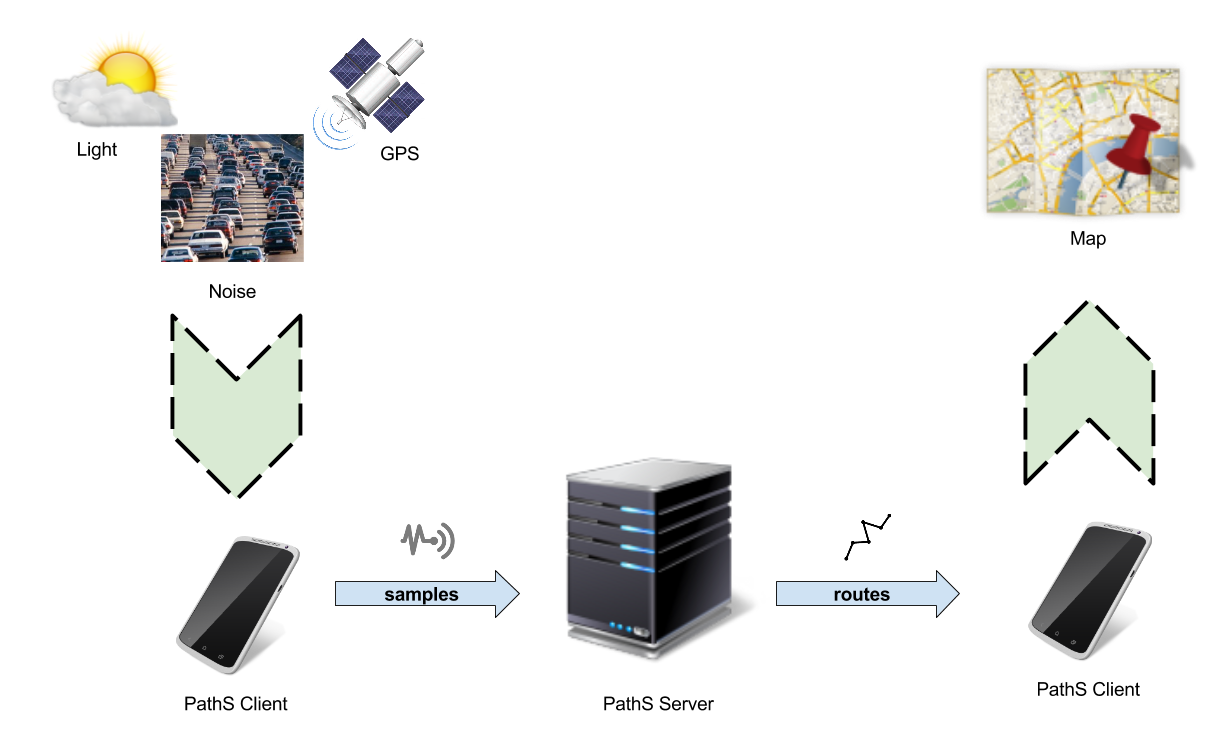
\includegraphics[width=12cm]{paths-general}
  \caption{\footnotesize{Schema generale del progetto PathS.}}
  \label{fig:paths-general}
\end{figure}

Considerati questi aspetti, ed in particolare le difficoltà nell'estendere il progetto esistente;  con il gruppo di lavoro si è cercato di ridefinire i requisiti del sistema ponendo l'attenzione su alcuni punti principali, ovvero:
\begin{itemize}
\item \textbf{raccolta campioni}: il sistema deve ricevere i campioni dalle applicazioni \emph{client} in un formato ben definito e dalle possibilità di estensione;
\item \textbf{persistenza}: il sistema deve memorizzare in modo efficiente e coerente le informazioni ricevute relative ai campioni di tipologia diversa;
\item \textbf{associazione dei campioni ai percorsi}: il sistema deve eseguire l'operazione di associazione delle informazioni raccolte dai sistemi client (sensori) alle informazioni di geolocalizzazione e cartografia (strade);
\item \textbf{routing}: il sistema deve implementare un servizio di calcolo dei percorsi pedonali complesso che rielabori le informazioni precedentemente raccolte;
\item \textbf{interfacciamento con il client}: il sistema deve comunicare con le applicazioni \emph{mobile} fornendo le informazioni necessarie alla navigazione.
\end{itemize}

Oltre a questi requisiti fondamentali per il funzionamento del sistema, sono stati individuati altri criteri preferibili di carattere qualitativo da considerare nella progettzione e implementazioone del software. Si possono riassumere in:
\begin{itemize}
\item \textbf{suddivisione delle responsabilità}: delineare in modo specifico le funzioni svolte da ciascun componente del sistema, evitando elementi che svolgono funzioni troppo complesse o che accoppiano troppi elementi. Questo approccio consente una migliore testabilità delle sotto-componenti e la possibilità di rivedere e riprogettare alcuni dettagli senza dover manipolare l'intero software;
\item \textbf{astrazione}: identificare la funzione logica di ciascun componente prima di concentrarsi sull'implementazione. Questo consente di delineare con precisione il ruolo che dovrà svolgere, precondizioni e risultati. Rispettare questo criterio dovrebbe rendere più facile la riscrittura o il miglioramento dell'implementazione dei componenti senza doverne ridefinire la funzione logica;
\item \textbf{estensibilità}: rendere agevole sia intrmine architetturali che implementativi la possibilità di migliorare ed estendere il sistema. L'obiettivo del progetto è stato volutamente limitato ad un primo risultato tangibile, considerando però che vi sia la possibilità di migliorare ed estendere le sue parti in modo facile e coerente con la base che si andrà a sviluppare.
\end{itemize}

\section{Componenti}
Identificazione delle componenti logiche del server sulla base delle funzioni che deve svolgere.
\subsection{Ricezione dei campioni}
La componente di ricezione campioni deve colloquiare con il client. Necessità di definire un formato chiaro e \emph{standard}, facilmente implementabile con qualsiasi tecnologia \emph{client} ed eventualmente da altri sorgenti dati.
\subsection{Elaborazione dei campioni}
I campioni così come sono ricevuti dai client sono in formato grezzo e non consentono di sfruttare le inormazioni in esse contenute. Il passo principale per l'utilizzo dei dati è quello di associare ciascun dato ad un segmento della rete di trasporto. 
\subsection{Interrogazione}
Lo scopo pensato per l'utilizzo delle informazioni raccolte è quello di fornire servizi \emph{routing} alternativi, che tengano conto dei dati raccolti per suggerire percorsi che vanno oltre la semplice regola del percorso più breve. Il componente deve quindi:
\begin{itemize}
\item definire un formato di colloquio con il client per i percorsi;
\item implementare un algoritmo di routing;
\item modificare l'algoritmo di routing affinché consideri le informazioni aggiuntive.
\end{itemize}

\section{Tecnologie e linee guida}
Tecnologie e librerie selezionate per l'applicazione globale al sistema server (Play! Framework, PostgresSQL, LeafletJS, Bootstrap). Linee guida di utilizzo delle tecnologie per rispettare i requisiti non funzionali.